\chapter{\textit{DYNAMIC TIME WARPING}} \label{cha:dtw}

O Dynamic Time Warping (DTW) é um algoritmo amplamente utilizado para medir a similaridade entre duas sequências temporais que podem variar em velocidade, tempo ou comprimento. Sua principal aplicação está em áreas como reconhecimento de fala, análise de séries temporais, bioinformática e visão computacional. Neste trabalho, o DTW é utilizado como ferramenta para comparação entre as curvas que representam as características faciais dos indivíduos, permitindo identificar semelhanças de mesmas pessoas em diferentes momentos ou condições.

\section{Introdução ao DTW}

O DTW surgiu como uma solução para o problema de comparação entre sequências temporais que apresentam distorções no eixo do tempo. Diferente da distância Euclidiana, que compara ponto a ponto, o DTW permite alinhar dinamicamente duas sequências, encontrando o menor custo de distorção temporal necessário para que elas se assemelhem.

Considere duas sequências temporais:

\begin{equation}
    X = (x_1, x_2, \ldots, x_n) \quad \text{e} \quad Y = (y_1, y_2, \ldots, y_m)
\end{equation}
onde \(X\) e \(Y\) são as sequências a serem comparadas, com \(n\) e \(m\) sendo seus respectivos comprimentos. O DTW constrói uma matriz de custo \(D\) de tamanho \(n \times m\), onde cada elemento \(D(i, j)\) representa o custo acumulado para alinhar os primeiros \(i\) elementos de \(X\) com os primeiros \(j\) elementos de \(Y\).

A matriz de custo é preenchida de forma recursiva, considerando o custo mínimo para cada posição \(D(i, j)\):
\begin{equation}
    D(i, j) = d(x_i, y_j) + \min \begin{cases}
        D(i-1, j) \\
        D(i, j-1) \\
        D(i-1, j-1)
    \end{cases}
\end{equation}
onde \(d(x_i, y_j)\) é a distância entre os pontos \(x_i\) e \(y_j\). O custo total do alinhamento é obtido em \(D(n, m)\).

A \autoref{fig:dtw_intro} ilustra o conceito de alinhamento dinâmico, mostrando como o DTW pode distorcer o eixo do tempo para alinhar duas sequências temporais que, à primeira vista, parecem diferentes.

\begin{figure}[h!]
    \centering
    \caption{ALINHAMENTO DINÂMICO.}
    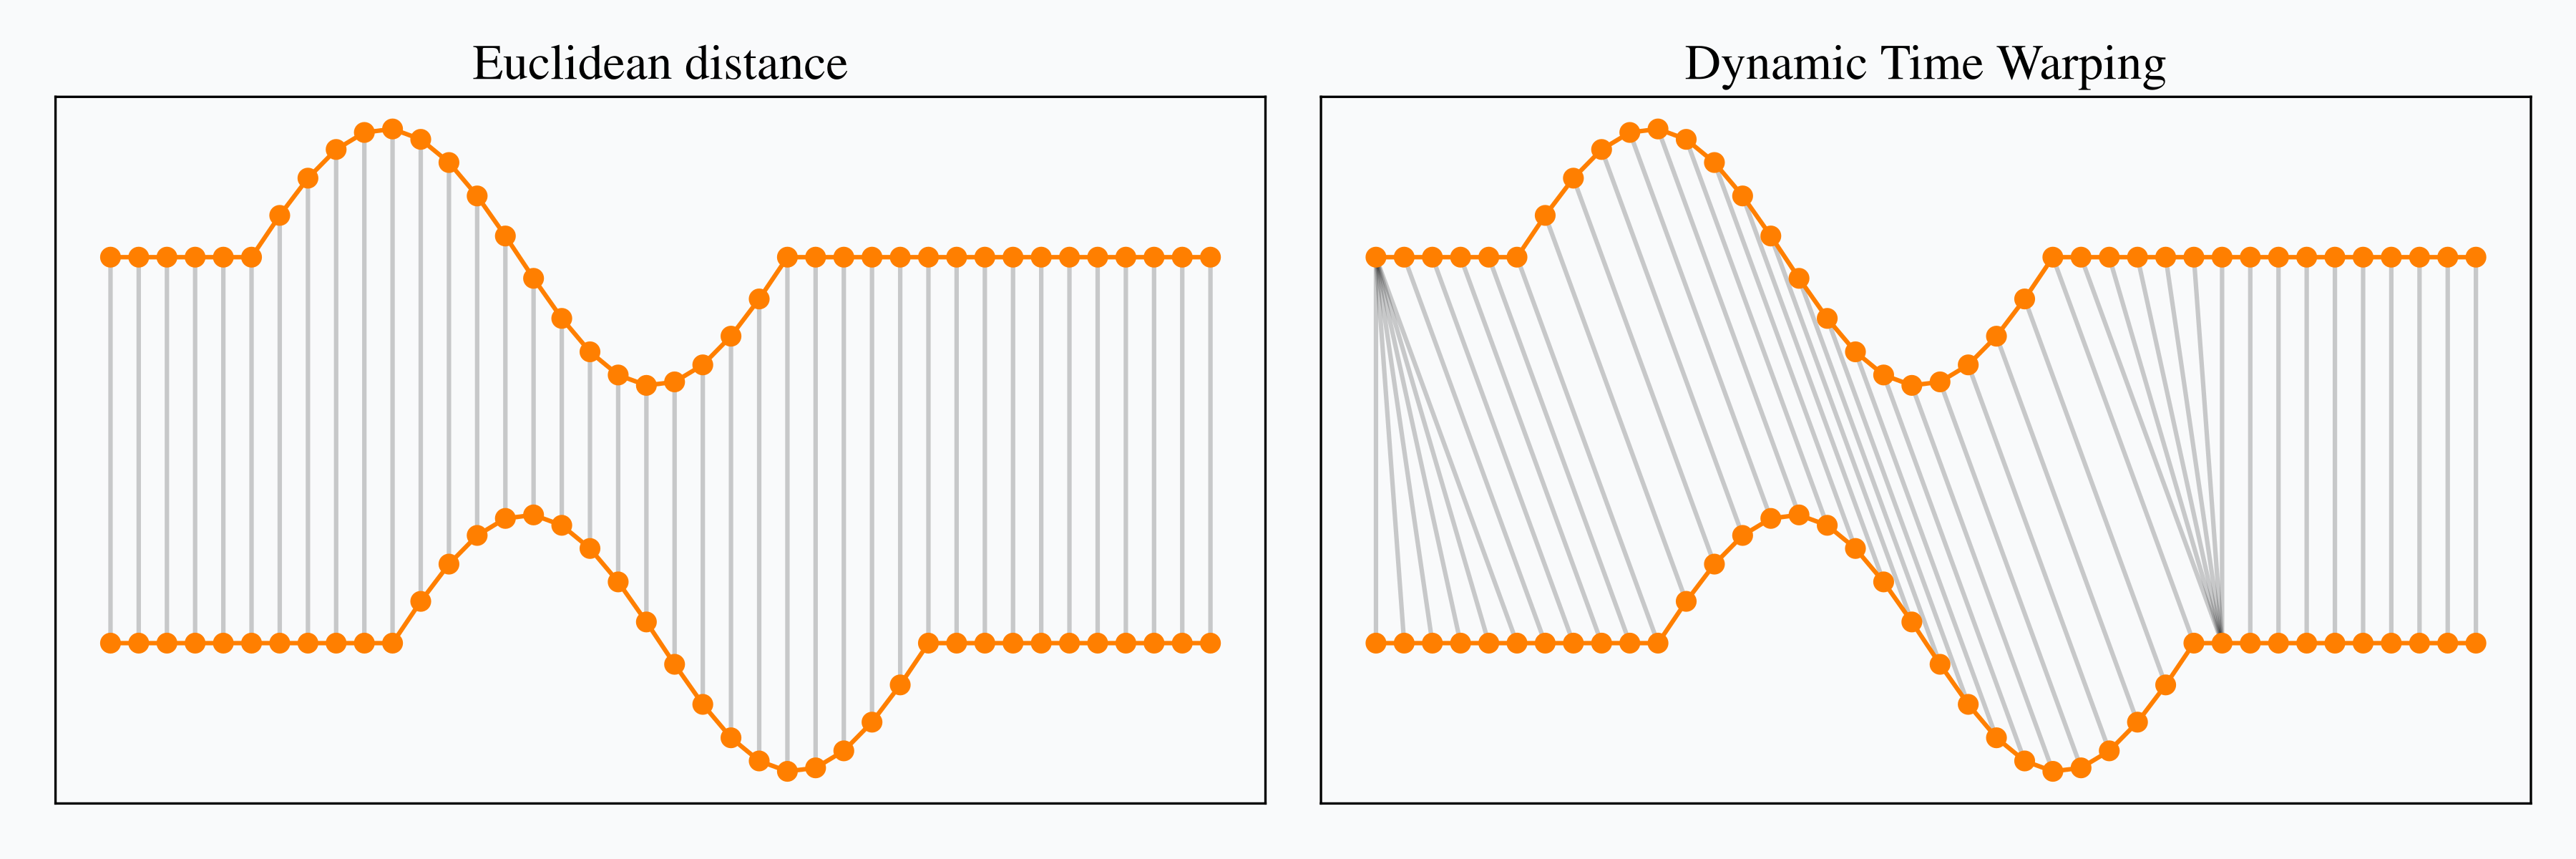
\includegraphics[width=0.8\textwidth]{fig/dtw_vs_euc.png}
    \legend{FONTE: \cite{tavenard.blog.dtw}}
    \label{fig:dtw_intro}
\end{figure}

\section{Vantagens e Desvantagens do DTW}

O DTW apresenta diversas vantagens em relação a outras métricas de distância, como a distância Euclidiana. Entre elas, destacam-se:
\begin{itemize}
    \item \textbf{Robustez a variações de tempo}: O DTW é capaz de lidar com sequências que apresentam variações na velocidade ou no comprimento, permitindo comparações mais precisas.
    \item \textbf{Alinhamento dinâmico}: O DTW encontra o melhor alinhamento entre as sequências, minimizando o custo total de distorção temporal.
    \item \textbf{Versatilidade}: Funciona bem em sinais unidimensionais e multidimensionais, sendo aplicável em diversas áreas como reconhecimento de padrões e análise de séries temporais.
\end{itemize}

No entanto, o DTW também possui desvantagens:
\begin{itemize}
    \item \textbf{Complexidade computacional}: O algoritmo tem complexidade \(O(n \cdot m)\), o que pode ser um limitante para sequências muito longas.
    \item \textbf{Sensibilidade a ruídos}: O DTW pode ser afetado por ruídos nas sequências, o que pode levar a alinhamentos incorretos.
\end{itemize}


\section{Justificativa para o uso do DTW}

Neste trabalho, o DTW foi utilizado por ser uma técnica adequada para comparar sequências que representam características espaciais extraídas de contornos faciais utilizando um algoritmo simples. As curvas resultantes dessas características podem variar em comprimento e forma devido a diferentes condições de iluminação, expressões faciais ou ângulos de captura. O DTW permite alinhar essas curvas de forma dinâmica, possibilitando uma comparação mais precisa entre elas.

Além disso, este trabalho se baseia na abordagem proposta por \citet{DTW_LSTM}, que demonstrou a eficácia do uso do DTW na comparação da variação das cores dos pixels, alcançando acurácias superiores a 90\% em tarefas de reconhecimento facial. No entanto, uma limitação observada nesse estudo foi o elevado custo computacional associado ao DTW, o que o torna menos viável para aplicações em tempo real. 

Diante disso, uma das propostas deste trabalho é otimizar o processo de comparação por meio da utilização de curvas suaves representadas por splines, com o objetivo de reduzir a complexidade computacional sem comprometer a acurácia e a eficiência da técnica.